\section{Transferring a crossing to an inner system}
\label{sec:transfer}

Fix a bucket of a driver and restrict physical time to \(0\le x\le1\).
Its canonical readings \(s,u\) give three feasible inner points with
the same time \(w=s-u\), one for each of \(Q_A,Q_C,Q_R\)
in~\eqref{eq:driver-memberships}. To use an inner crossing bound, we
must also transfer admissibility and control the number of segments
in the resulting path. The two clock vectors use coordinates of the
driver itself. The resource vector uses minima of scheduler slacks,
so its admissibility requires a separate dimension argument.

\subsection{Transferring admissibility}

\begin{lemma}[Clock readings]\label{lem:transfer}
At an admissible driver point, inactivity of the bucket implies
\[
                    |w-(a(x)-c(x))|\le 2C_*\rho .
\]
If every coordinate of \(A\) exceeds \(a(x)\), the bucket is active
and \((w,z_A)\) is admissible for \(Q_A\). The corresponding assertion
holds for \(C,c(x),Q_C\). For \(1/4\le w\le3/4\), the \(A\) assertion
applies in the early phase and the \(C\) assertion in the late phase.
\end{lemma}

\begin{proof}
Fix a usable set certifying admissibility in
Definition~\ref{def:admissible}. Its coordinates in each clock copy form
a viable set for that copy, of size greater than \(J\). If the bucket
were inactive and every \(A\) floor were slack, no tight driver row
would involve \(A\). The usable \(A\) coordinates alone would then
supply more than \(J\) independent kernel directions. Thus in an
inactive bucket some \(A\) floor is attained, and likewise some
\(C\) floor is attained. The two minima equal \(a(x)\) and \(c(x)\),
respectively. These are below the cap \(T_*\), so subtracting the two
estimates in~\eqref{eq:canonical-estimate} gives the reading bound.

Now suppose that every \(A\) floor is slack. The bucket is active.
Every tight \(Q_A\) row occurs in a tight coupling row by
Lemma~\ref{lem:coupling}. The multiplier of its \(A\) normal is
positive and its support is therefore usable. Take a variation on
the usable \(A\) coordinates in the common kernel of these inner
normals and extend it by zero on all other coordinates. It annihilates
each tight driver row. Indeed, the only tight rows that can involve
\(A\) are coupling rows of this bucket, and their \(A\) parts are zero
or positive multiples of tight \(Q_A\) normals. The inner kernel thus
has dimension at most \(J\), as required. The proof for \(C\) is the
same with the two clocks interchanged.

In the early phase \(a-c=0\). If an \(A\) floor is attained,
\(s\le a+C_*\rho\), while \(u\ge c-C_*\rho\) always. Hence
\(w\le2C_*\rho<1/4\). In the late phase \(a-c=1\). Attainment
of a \(C\) floor would give \(w\ge1-2C_*\rho>3/4\).
\end{proof}

\begin{lemma}[Resource transfer]\label{lem:resource-transfer}
At every admissible driver point in the probe band of the bucket,
the bucket is active and \((w,z_R)\) is admissible for \(Q_R\).
\end{lemma}

\begin{proof}
Fix a certificate of driver admissibility. Its set \(I\) of usable
scheduler coordinates is viable for the scheduler. At the given
physical time \(x\), let \(\mathcal W\) consist of all tight non-red
scheduler rows together with every red row used in a tight coupling
row of any bucket. Count each row identity only once. Each of these
rows is supported on \(I\). For a used red row this follows from the
strictly positive coefficient of its slack and the nonnegativity of
all normals in the coupling.

\paragraph{Completing the tight equalities.}
Restrict the scheduler slice to \(I\). Keep the non-red bounds, move
each used red bound to equality at the given point, and relax any
other violated red bound just enough to make the point feasible.
Lemma~\ref{lem:active} bounds every change by \(O(\tau)\). We chose
\(\tau\) small enough for these perturbations to lie within the
tolerance in Theorem~\ref{thm:scheduler}. The rows in \(\mathcal W\)
are now tight at a feasible point. Their normals are independent
on \(I\), since the point lies in the probe band and perturbing the
bounds leaves their normals unchanged. Consequently the linear map
\[
       L:\mathbb R^I\longrightarrow\mathbb R^{\mathcal W},
       \qquad \delta z\longmapsto
       (\text{variation of the slack of row }h)_{h\in\mathcal W}
\]
is onto, with kernel dimension \(j_0=|I|-|\mathcal W|\). Every
variation in its kernel, extended by zero outside \(I\), fixes all
tight driver rows. Thus \(j_0\le J\).

The face of the perturbed slice defined by \(\mathcal W\) is nonempty
and pointed. Choose one of its vertices. At this vertex the tight
normals span \(\mathbb R^I\) and are independent, so there are exactly
\(j_0\) tight rows besides \(\mathcal W\). Write \(U_0\) for the
requests of our bucket represented by red rows in \(\mathcal W\),
and \(U\) for the requests of that bucket represented by all tight
red rows at the vertex. Then
\[
              U_0\subseteq U,\qquad |U\setminus U_0|\le j_0 .
\]
The vertex of the perturbed slice supplies the set \(U\) for testing
admissibility at the original resource point. The scheduler's vertex
guarantee gives viability of \(U\) for the client program, and hence \(|U|>J\). In particular \(U_0\ne\varnothing\).
A red row contributing to \(U_0\) was used by a tight coupling of this
bucket at the original point, proving activity there.

\paragraph{Accounting for the added requests.}
At the original point, every tight resource row occurs in a tight
coupling by Lemma~\ref{lem:coupling}. The red rows in that coupling
represent all requests in the resource row's support, so every such
support lies in \(U_0\). Let \(H\subseteq\mathbb R^{U_0}\) be the
common kernel of the tight resource normals restricted to \(U_0\).
For \(v\in H\), assign slack variation \(v_i\) to every row in
\(\mathcal W\) representing request \(i\) of this bucket. Assign zero
to all other rows of \(\mathcal W\). This embeds \(H\) in
\(\mathbb R^{\mathcal W}\), since each \(i\in U_0\) is represented.
By surjectivity of \(L\), the inverse image of this embedded subspace
has dimension \(j_0+\dim H\).

The variations in this inverse image annihilate all tight driver rows
when every coordinate outside \(I\) is held fixed. Tight non-red
slacks and slacks used by other buckets stay fixed. In a tight
coupling of our bucket, the scheduler contribution varies by
\(b_R\cdot v/\tau=0\), where \(b_R\) is its tight resource normal.
All choices of a representative of request \(i\) give the same
variation \(v_i\). Driver admissibility therefore gives
\(j_0+\dim H\le J\). On the viable set \(U\) the resource kernel
has dimension
\[
         \dim H+|U\setminus U_0|\ \le\ \dim H+j_0\ \le\ J,
\]
because the newly added coordinates lie outside every tight resource
support. This proves admissibility at \((w,z_R)\).
\end{proof}

\subsection{Straightening the transferred path}

The three transfers are continuous. Even on a straight segment of the
driver, the red row attaining a given minimum can change many times.
The following lemma bounds the cost of all such changes at once.

\begin{lemma}[Two-chord straightening]\label{lem:two-chords}
Fix a transfer which applies throughout an affine segment of
admissible driver points with the bucket active. Its inner endpoints
can be joined by an admissible path preserving the reading at every
parameter. One segment suffices for a clock transfer and at most
two for a resource transfer.
\end{lemma}

\begin{proof}
Choose a coupling row tight at the midpoint. Its affine slack on the
driver segment is nonnegative and vanishes there, hence vanishes on
the entire segment. Its two upper equalities determine \(s,u\)
affinely by Lemma~\ref{lem:coupling}. Thus \(w\) and both clock
images are affine. The assumed clock transfer certifies admissibility
pointwise, so a clock image itself is the desired segment.

For the resource transfer each coordinate of \(\mu\) is a minimum of
affine functions along the segment. Therefore each coordinate of
\(z_R\) is concave. Every resource row has nonnegative coordinate
normal and its right-hand side is affine in \(w\), so its slack along
the resource image is a nonnegative concave function. Such a function
vanishing at any interior parameter vanishes everywhere. Thus all
interior points of the image have precisely the tight rows of its
midpoint, and both endpoints satisfy these rows with equality.

Replace the image by two chords, one joining each endpoint to the
midpoint. They are feasible because the inner system is convex in
the joint variables \((w,z_R)\). On the open part of each chord an
affine nonnegative slack is zero exactly when it is zero at both
ends of that chord. These common equalities are precisely the
midpoint's tight rows. Its usable set certifies the two open chords,
and the three retained points keep their original certificates.
Since \(w\) is affine, the chords preserve it pointwise.
\end{proof}

One chord can introduce additional tight rows. For example, take
\(a,b,c\ge0\), \(a+b\ge1\), \(J=0\), and a program for which any
one of the three coordinates is viable
(Section~\ref{sec:framework}). On the broken line
\[
               (1,0,0)\ \longrightarrow\ (1,1,0)\
                         \longrightarrow\ (0,1,0)
\]
the endpoints are vertices and every interior point has only the
equality \(c=0\). With the bend halfway along the parameter interval,
the image is coordinatewise concave. The direct chord between the
endpoints would impose \(a+b=1\) as well as \(c=0\). Their supports
require all three coordinates to be usable, yet the two normals have
nullity one on these coordinates. Retaining the middle point avoids
this additional equality.

\paragraph{The cost of a work window.}
Suppose a driver subpath meets both reading endpoints of a work window
and its transfer applies over the portion used to cross. Orient the
subpath so it visits the near endpoint first. Stop at the first far
endpoint visit after that, and begin at the last near endpoint visit
before the stopping time. By continuity the trimmed reading remains
in the closed window. Restrict the given segmentation to this subpath
and apply Lemma~\ref{lem:two-chords} to each resulting segment. The
replacements agree at their endpoints. Throughout the window,
Lemma~\ref{lem:overlay} identifies the overlay with the input by an
affine translation and time change. This preserves the coordinate
normals of the tight rows, their supports, and the request program,
so the resulting polygonal path is an admissible input crossing.
It has at most as many segments as the trimmed driver path for a
clock transfer, and at most twice that number for a resource transfer.
The input requires \(D_*\) segments. In either case at least
\(D_*/2-1\) breaks of the given segmentation lie strictly inside
the trimmed path. Cutting at its two endpoints contributes no breaks
to this count.

\subsection{Counting traversals of an episode}

\begin{figure}[htbp]
\centering
\definecolor{episodeink}{RGB}{35,91,101}
\definecolor{episodetrace}{RGB}{137,67,36}
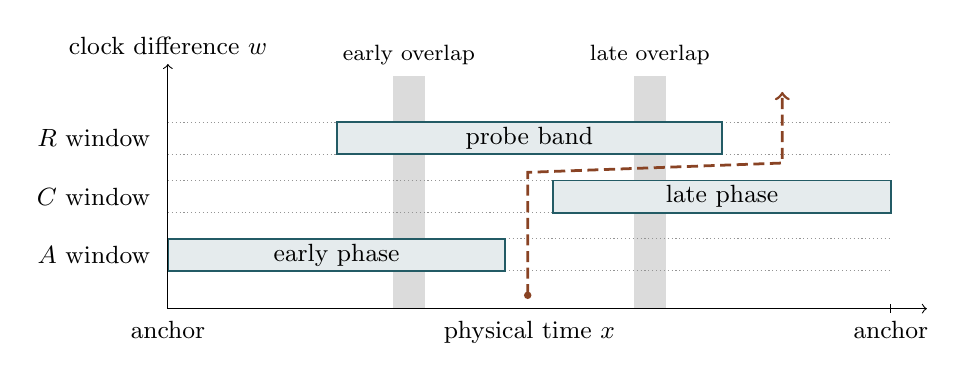
\begin{tikzpicture}[x=1.02cm,y=.74cm,font=\small,
  bar/.style={draw=episodeink,fill=episodeink!12,line width=.7pt},
  trace/.style={draw=episodetrace,line width=1pt,dash pattern=on 4pt off 2pt}]
  % A fixed bucket in one episode. Vertical strips are in x; rows are in w.
  \foreach \x in {2.8,5.8}{
    \fill[black!14] (\x,0) rectangle (\x+.4,4);
  }
  \foreach \y in {.65,1.65,2.65}{
    \draw[black!42,densely dotted] (0,\y) -- (9,\y);
    \draw[black!42,densely dotted] (0,\y+.55) -- (9,\y+.55);
  }

  \draw[bar] (0,.65) rectangle (4.2,1.20);
  \draw[bar] (4.8,1.65) rectangle (9,2.20);
  \draw[bar] (2.1,2.65) rectangle (6.9,3.20);
  \node at (2.10,.925) {early phase};
  \node at (6.90,1.925) {late phase};
  \node at (4.50,2.925) {probe band};
  \node[anchor=east] at (-.10,.925) {\(A\) window};
  \node[anchor=east] at (-.10,1.925) {\(C\) window};
  \node[anchor=east] at (-.10,2.925) {\(R\) window};

  \draw[trace,->] (4.48,.23) -- (4.48,2.34) -- (7.65,2.5) -- (7.65,3.72);
  \fill[episodetrace] (4.48,.23) circle (1.35pt);
  \draw[->] (0,0) -- (0,4.2) node[above] {clock difference \(w\)};
  \draw[->] (0,0) -- (9.45,0);
  \draw (9,.08) -- (9,-.08);
  \node[below] at (0,-.05) {anchor};
  \node[below] at (9,-.05) {anchor};
  \node[below] at (4.5,-.05) {physical time \(x\)};
  \node[anchor=south,font=\footnotesize] at (3.0,4.02) {early overlap};
  \node[anchor=south,font=\footnotesize] at (6.0,4.02) {late overlap};
\end{tikzpicture}
\caption{One bucket and one ordered triple of work windows. The rectangle
in each horizontal window marks the physical times when its transfer is
guaranteed. The dashed subpath spans the triple in \(w\) while missing all
three rectangles. Its \(x\)-coordinate traverses the shaded late overlap
as it moves from the \(C\) window to the \(R\) window.}
\label{fig:episode}
\end{figure}


The phases and probe band in Figure~\ref{fig:episode} are intervals
of physical time \(x\). The work windows lie on a second axis, the
reading \(w\). A crossing in \(w\) gives the segment bound just proved
if \(x\) stays in the corresponding phase or band. If \(x\) ranges
farther, it must traverse a physical overlap which can host a new
episode.

\begin{lemma}[Episode traversal]\label{lem:episode}
Fix any segmentation of an admissible traversal of an episode which
stays between the anchors and reaches them in either order. It
contains \(q_*\) subpaths with disjoint parameter interiors. Each
subpath has at least \(D_*/2-1\) interior breaks or contains a
traversal of one of the episode's \(2B\) designated overlaps that
stays inside that overlap.
\end{lemma}

\begin{proof}
Orient the path from the early anchor to the late anchor. At most
\(2Vm\) buckets are active at either anchor by Lemma~\ref{lem:active}.
Since \(B>4Vm\), one bucket is inactive at both. Its reading starts
below \(1/4\) and ends above \(3/4\) by Lemma~\ref{lem:transfer}.

For each ordered triple of work windows, stop at the first time
\(w\) hits its rightmost endpoint and trim back to the last time
\(w\) hits its leftmost endpoint before then. On the intervening
subpath \(w\) stays in the span of the triple. Each later triple
lies strictly to the right of the preceding triple. Its leftmost
endpoint can first be reached only after the preceding rightmost
endpoint has been reached, so the subpaths have disjoint interiors.

Consider the physical times \(x\) visited on one such subpath.
If they all lie in the early phase, the late phase, or the probe band,
apply the \(A\), \(C\), or \(R\) transfer, respectively. The subpath
crosses the corresponding work window inside the triple and hence
contains at least \(D_*/2-1\) interior breaks.

Otherwise the physical range lies in none of the three intervals.
If it contains a point before the band, it also contains a point
after the end of the early phase. The entire designated early overlap
lies strictly between those physical times. If the range contains
a point after the band, it also contains a point before the start
of the late phase, with the late overlap strictly between them.
At least one of these cases occurs. Trim between visits to the
endpoints of that overlap, reversing the orientation if necessary,
to obtain a traversal staying inside it. Backtracking in either
\(x\) or \(w\) is allowed throughout. Even when two subpaths reach
the same physical overlap, they visit it on disjoint parameter
interiors.
\end{proof}
